\documentclass{article}
\twocolumn
\usepackage{proof}
\usepackage{tikz}
\usepackage{hyperref}
\usepackage{chngcntr}
\usepackage{microtype}
\usepackage{subcaption}
\counterwithin{figure}{section}

\usetikzlibrary{fit,automata,positioning}
%%%%%%%%%%%%%%%%%%%%%%%%%%%%%%%%%%%%%%%%%
% Lachaise Assignment
% Structure Specification File
% Version 1.0 (26/6/2018)
%
% This template originates from:
% http://www.LaTeXTemplates.com
%
% Authors:
% Marion Lachaise & François Févotte
% Vel (vel@LaTeXTemplates.com)
%
% License:
% CC BY-NC-SA 3.0 (http://creativecommons.org/licenses/by-nc-sa/3.0/)
% 
%%%%%%%%%%%%%%%%%%%%%%%%%%%%%%%%%%%%%%%%%

%----------------------------------------------------------------------------------------
%	PACKAGES AND OTHER DOCUMENT CONFIGURATIONS
%----------------------------------------------------------------------------------------

\usepackage{amsmath,amsfonts,stmaryrd,amssymb} % Math packages

\usepackage{enumerate} % Custom item numbers for enumerations

\usepackage[ruled]{algorithm2e} % Algorithms

\usepackage[framemethod=tikz]{mdframed} % Allows defining custom boxed/framed environments

\usepackage{listings} % File listings, with syntax highlighting
\lstset{
	basicstyle=\ttfamily, % Typeset listings in monospace font
}

%----------------------------------------------------------------------------------------
%	DOCUMENT MARGINS
%----------------------------------------------------------------------------------------

\usepackage{geometry} % Required for adjusting page dimensions and margins

\geometry{
	paper=a4paper, % Paper size, change to letterpaper for US letter size
	top=2.5cm, % Top margin
	bottom=3cm, % Bottom margin
	left=2.5cm, % Left margin
	right=2.5cm, % Right margin
	headheight=14pt, % Header height
	footskip=1.5cm, % Space from the bottom margin to the baseline of the footer
	headsep=1.2cm, % Space from the top margin to the baseline of the header
	%showframe, % Uncomment to show how the type block is set on the page
}

%----------------------------------------------------------------------------------------
%	FONTS
%----------------------------------------------------------------------------------------

\usepackage[utf8]{inputenc} % Required for inputting international characters
\usepackage[T1]{fontenc} % Output font encoding for international characters

\usepackage{XCharter} % Use the XCharter fonts

%----------------------------------------------------------------------------------------
%	COMMAND LINE ENVIRONMENT
%----------------------------------------------------------------------------------------

% Usage:
% \begin{commandline}
%	\begin{verbatim}
%		$ ls
%		
%		Applications	Desktop	...
%	\end{verbatim}
% \end{commandline}

\mdfdefinestyle{commandline}{
	leftmargin=10pt,
	rightmargin=10pt,
	innerleftmargin=15pt,
	middlelinecolor=black!50!white,
	middlelinewidth=2pt,
	frametitlerule=false,
	backgroundcolor=black!5!white,
	frametitle={Command Line},
	frametitlefont={\normalfont\sffamily\color{white}\hspace{-1em}},
	frametitlebackgroundcolor=black!50!white,
	nobreak,
}

% Define a custom environment for command-line snapshots
\newenvironment{commandline}{
	\medskip
	\begin{mdframed}[style=commandline]
}{
	\end{mdframed}
	\medskip
}

%----------------------------------------------------------------------------------------
%	FILE CONTENTS ENVIRONMENT
%----------------------------------------------------------------------------------------

% Usage:
% \begin{file}[optional filename, defaults to "File"]
%	File contents, for example, with a listings environment
% \end{file}

\mdfdefinestyle{file}{
	innertopmargin=1.6\baselineskip,
	innerbottommargin=0.8\baselineskip,
	topline=false, bottomline=false,
	leftline=false, rightline=false,
	leftmargin=2cm,
	rightmargin=2cm,
	singleextra={%
		\draw[fill=black!10!white](P)++(0,-1.2em)rectangle(P-|O);
		\node[anchor=north west]
		at(P-|O){\ttfamily\mdfilename};
		%
		\def\l{3em}
		\draw(O-|P)++(-\l,0)--++(\l,\l)--(P)--(P-|O)--(O)--cycle;
		\draw(O-|P)++(-\l,0)--++(0,\l)--++(\l,0);
	},
	nobreak,
}

% Define a custom environment for file contents
\newenvironment{file}[1][File]{ % Set the default filename to "File"
	\medskip
	\newcommand{\mdfilename}{#1}
	\begin{mdframed}[style=file]
}{
	\end{mdframed}
	\medskip
}

%----------------------------------------------------------------------------------------
%	NUMBERED QUESTIONS ENVIRONMENT
%----------------------------------------------------------------------------------------

% Usage:
% \begin{question}[optional title]
%	Question contents
% \end{question}

\mdfdefinestyle{question}{
	innertopmargin=1.2\baselineskip,
	innerbottommargin=0.8\baselineskip,
	roundcorner=5pt,
	nobreak,
	singleextra={%
		\draw(P-|O)node[xshift=1em,anchor=west,fill=white,draw,rounded corners=5pt]{%
		Question \theQuestion\questionTitle};
	},
}

\newcounter{Question} % Stores the current question number that gets iterated with each new question

% Define a custom environment for numbered questions
\newenvironment{question}[1][\unskip]{
	\bigskip
	\stepcounter{Question}
	\newcommand{\questionTitle}{~#1}
	\begin{mdframed}[style=question]
}{
	\end{mdframed}
	\medskip
}

%----------------------------------------------------------------------------------------
%	WARNING TEXT ENVIRONMENT
%----------------------------------------------------------------------------------------

% Usage:
% \begin{warn}[optional title, defaults to "Warning:"]
%	Contents
% \end{warn}

\mdfdefinestyle{warning}{
	topline=false, bottomline=false,
	leftline=false, rightline=false,
	nobreak,
	singleextra={%
		\draw(P-|O)++(-0.5em,0)node(tmp1){};
		\draw(P-|O)++(0.5em,0)node(tmp2){};
		\fill[black,rotate around={45:(P-|O)}](tmp1)rectangle(tmp2);
		\node at(P-|O){\color{white}\scriptsize\bf !};
		\draw[very thick](P-|O)++(0,-1em)--(O);%--(O-|P);
	}
}

% Define a custom environment for warning text
\newenvironment{warn}[1][Warning:]{ % Set the default warning to "Warning:"
	\medskip
	\begin{mdframed}[style=warning]
		\noindent{\textbf{#1}}
}{
	\end{mdframed}
}

%----------------------------------------------------------------------------------------
%	INFORMATION ENVIRONMENT
%----------------------------------------------------------------------------------------

% Usage:
% \begin{info}[optional title, defaults to "Info:"]
% 	contents
% 	\end{info}

\mdfdefinestyle{info}{%
	topline=false, bottomline=false,
	leftline=false, rightline=false,
	nobreak,
	singleextra={%
		\fill[black](P-|O)circle[radius=0.4em];
		\node at(P-|O){\color{white}\scriptsize\bf i};
		\draw[very thick](P-|O)++(0,-0.8em)--(O);%--(O-|P);
	}
}

% Define a custom environment for information
\newenvironment{info}[1][Info:]{ % Set the default title to "Info:"
	\medskip
	\begin{mdframed}[style=info]
		\noindent{\textbf{#1}}
}{
	\end{mdframed}
}


\usepackage{listings}
\usepackage{color}

\definecolor{dkgreen}{rgb}{0,0.6,0}
\definecolor{gray}{rgb}{0.5,0.5,0.5}
\definecolor{mauve}{rgb}{0.58,0,0.82}

\lstset{frame=tb,
  language=Java,
  aboveskip=3mm,
  belowskip=3mm,
  showstringspaces=false,
  columns=flexible,
  basicstyle={\small\ttfamily},
  numbers=none,
  numberstyle=\tiny\color{gray},
  keywordstyle=\color{blue},
  commentstyle=\color{dkgreen},
  stringstyle=\color{mauve},
  breaklines=true,
  breakatwhitespace=true,
  tabsize=3
} 

\title{Parsly: Procedureless Protocol Compiler\\
		\large A Software Engineering Approach to \\ Simplify Protocol Development Process} 

\author{Han Zheng\\ \texttt{tim.zheng@hivechat.org}} 
\date{ \today} 




\begin{document}
\maketitle 

\section{Introductions} % Unnumbered section
\subsection{The Cycle of Protocol Development}
\begin{figure}[h!]
\begin{center}
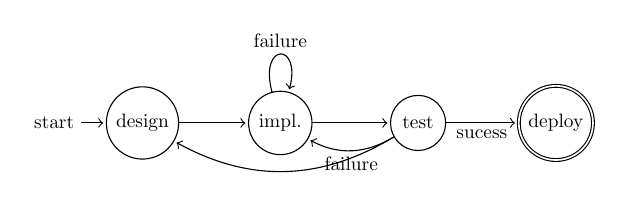
\begin{tikzpicture}[
	shorten >=1pt,
	node distance=2.5cm, 
	on grid, 
	auto, 
	scale=0.7, 
    transform shape, 
    align=center, 
    state/.style={
    	circle, 
    	draw, 
    	minimum size=1cm
    }] 
    
   \node[state,initial] (q_0)   {design}; 
   \node[state, right=of q_0] (q_1) {impl.}; 
   \node[state, right=of q_1] (q_2) {test}; 
   \node[state,accepting, right=of q_2](q_3) {deploy};
   \path[->] 
    (q_0) edge node {} (q_1)
    (q_1) edge node  {} (q_2)
    (q_1) edge [loop above] node {failure} (q_1)
    (q_2) edge node [swap] {sucess} (q_3) 
    (q_2) edge [bend left, below] node {failure} (q_1)
    (q_2) edge [bend left, below] node {} (q_0);
\end{tikzpicture}
\caption{development cycle}
\label{fig:developmentCycle}
\end{center}
\end{figure}

To better illustrate the process of protocol development, we divide it into four phases in a cycle: design, implement, test and deploy (see fig~\ref{fig:developmentCycle}). The devloper first need to design the message types and message fields of the protocol, and then implement the protocol with a programing language. Then the test phase comes, where the developer verifies that the implementation is correct. If the implementation is correct, the protocol is deployed, and the development can move on. Otherwise, the developer needs to go back and find out whether the problem lies in the design or the implementation. The implement phase usually turns out to be time consuming, as it involves noises like debugging and solving problems in the lower level protocols, like sticky packet of TCP.




\subsection{The Goal}

\begin{figure}[h!]
\begin{center}
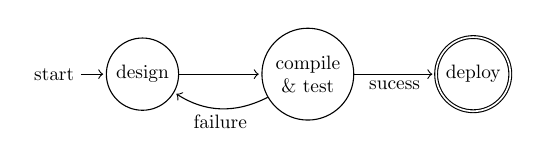
\begin{tikzpicture}[
	shorten >=1pt,
	node distance=3cm, 
	on grid, 
	auto, 
	scale=0.7, 
    transform shape, 
    align=center, 
    state/.style={
    	circle, 
    	draw, 
    	minimum size=1cm
    }] 
    
   \node[state,initial] (q_0)   {design}; 
   \node[state, right=of q_0] (q_2) {compile \\ \& test}; 
   \node[state,accepting, right=of q_2](q_3) {deploy};
   \path[->] 
    (q_0) edge node {} (q_2)
    (q_2) edge node [swap] {sucess} (q_3) 
    (q_2) edge [bend left, below] node {failure} (q_0);
\end{tikzpicture}
\caption{new development cycle}
\label{fig:newDevelopmentCycle}
\end{center}
\end{figure}

Protocol compiler is a tool that helps automate the process of network protocol implementation. It compiles a network protocol discriptions in a domain specific language (DSL), which declares message types and message fields, to a target programing language, like C++, Java and Python. This has saved programmer considerable amount of time by helping them to skip the implementation step, where programmers are prone to problems like nullpointer crash, sticky packet, serialization, and so on. Therefore, protocol compiler simplifies the development cycle into three simple phases (see fig~\ref{fig:newDevelopmentCycle})




\section{Limitation of Current Methods}

There are several protocol compilers that exists. The most commonly used one is Google's \textit{Protocol Buffers} (also known as \textit{protobuf}). Protobuf takes in a protocol declaration in their DSL called \textit{proto3} (fig~\ref{lst:proto3}) and generates the parsing logic in a popular collection of programing languages. During the runtime, \textit{protobuf} uses BSON, the binary representation of JavaScript Object Notation (JSON), to serialize and deserialise the messages. This has given programmers the convenience to handle the data by storing the message in JSON format.\\

However, there are several drawbacks in \textit{protobuf}. These drawbakcs mainly lies in the aspect of learning curve, performance, and correcness proving with formal verification.\\

First of all, although \textit{protobuf} has a well-designed DSL that concisely describes the protocol, it is one more language for the programer to learn and one more place to make mistakes. The programers need to read the documentations and do some practices in order to get started, which makes it harder to be used in fast-paced agile developent theme.\\

Speaking of performance, although \textit{protobuf} did a great job on space optimization by employing BSON for data serialization, BSON is not flexible enough for the users to tunne for optimization. Besides, \textit{protobuf} serializes message field type names into the message, which can be redundant therefore unnecessary. We will talk about this in section~\ref{subsec:performanceAnalysis} \\

Moreover, when it comes to proof driven deveolpment, where, in order to prove the correctness of the implementation of the protocol, the developer needs to get the formal specification of the DSL. However, the specificaiton is not officially available, and even if it will be available in the future, it means more work for the developer, as there is one more layer of language to reason about. \\


\section{Parsly}
Therefore we introduce parsly, a protocol compiler that compiles protocol descriptions in JSON to C++ parsing logics. Parsley implements a serialization method that is similar to the BSON format but gives user more freedom of space optimizations. \\

\subsection{Design}
Parsly is designed to be light-weight and portable, and works on UNIX operating systems as well as Windows. It consists of two parts, a C++ library called \textit{libagio} and a protocol compiler called \textit{pop}. Parsly implements this library (\textit{libagio}), which simplifies parsing logic for the compiler to easily work with. Taking the advantage of the modern C++ template, it is able to do many compile-time optimization for the serialization algorithms. As for the compiler, it is implemented in Python to achieve a high portability and lower cost of maintainance.  \\

\begin{figure}[h!]
\begin{center}
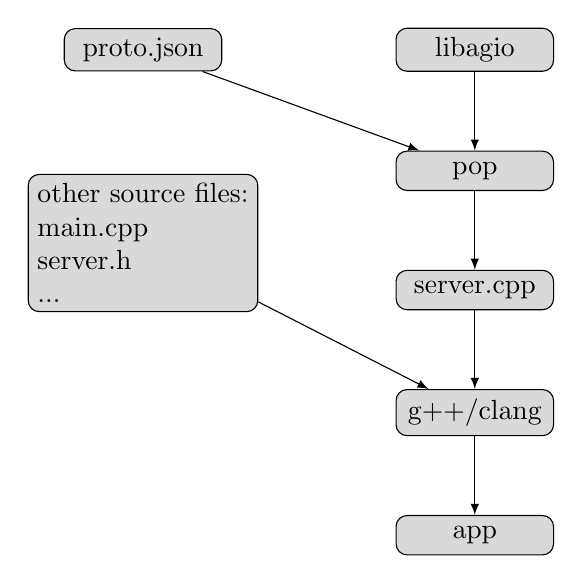
\begin{tikzpicture} [
	node distance = 7mm and -3mm,
	every node/.style = {
		draw=black, 
		rounded corners, 
		fill=gray!30, 
		minimum width=2cm, 
		minimum height=0.5cm,
		align=center
	},
	every path/.style = {draw, -latex}
]

\node (json) {proto.json};
\node (libagio) [right=2.2cm of json] {libagio};

\node (pop) [below=1cm of libagio] {pop};
\node (cpp) [below=1cm of pop] {server.cpp};
\node (srcs) [below=1.3cm of json, draw, align=left] {
other source files: \\ main.cpp\\ server.h\\ ...
};
\node (compiler) [below=1cm of cpp] {g++/clang};
\node (app) [below=1cm of compiler] {app};

\draw   (json) -> (pop);
\draw   (libagio) -> (pop);
\draw   (pop) -> (cpp);
\draw   (srcs) -> (compiler);
\draw   (cpp) -> (compiler);
\draw   (compiler) -> (app);

\end{tikzpicture}
\caption{build process}
\label{fig:builfProcess}
\end{center}
\end{figure}

To compile a network application, the user needs to go through three steps, see fig~\ref{fig:builfProcess}. First, design and write the protocol in JSON, with the attributes and formats provided by parsly. A working example is shown in fig~\ref{lst:parslyJson}. Then the user runs \textit{pop} by supplying the JSON protocol description and the target C++ output source file. \textit{Pop} will compile the protocol description into C++ code written with the \textit{libagio}'s API, and inject the code into the parsing function of the source file. The user is then able to run the C++ compiler to build the application.



\label{subsec:performanceAnalysis}
\subsection{Performance Analysis}
According to the BSON's \href{http://bsonspec.org}{documentation}, BSON is designed to be efficient in space, but in some cases it uses even more space than JSON because it adds the length indicator of strings and subobjects which makes traversal faster.\\

\begin{figure}[h!]
\begin{align*}
\text{document} :=&  \text{int32 e\_list "\textbackslash x00" } \\
\text{e\_list} :=& \text{element e\_list} \\
&| \ \text{""} \\
\text{element}	:=& \text{"\textbackslash x01" e\_name double} \\
&| \ \text{"\textbackslash x02" e\_name string} \\
&| \ \text{"\textbackslash x03" e\_name document} \\
&| \ \text{"\textbackslash x04" e\_name document} \\
&| \ \text{"\textbackslash x05" e\_name binary} \\
&| \ \cdots \\
\text{string} :=& \text{int32 (byte*) "\textbackslash x00"} \\
\text{binary} :=& \text{int32 subtype (byte*)} \\
\text{subtype} :=& \text{"\textbackslash x00"} \\
&| \ \text{"\textbackslash x01"} \\
&| \ \text{"\textbackslash x02"} \\
&| \ \cdots 
\end{align*}
\caption{BSON standard v1.1 grammar}
\label{eq:bsonGrammar}
\end{figure}

BSON uses 32-bit integer (int32) to indicate the length of the strings, binaries, as well as the document, and this is fixed by the specification, see fig~\ref{eq:bsonGrammar}. Therefore, no matter how long the string, binary or the document is, the length of the bytes that describes the data is fixed. This has left no space for user to optimize for space. For a message containing massive short strings, BSON will not perform well at all.  \\

\begin{figure}[h!]
\begin{align*}
M :=& \phi \ \text{e\_list} \\
\phi :=& \text{int8} \\
&| \ \text{int16} \\
&| \ \text{int32} \\
\text{e\_list} :=& \text{element } \text{e\_list}\\
&| \ \text{""} \\
\text{element}	:=& \text{unscoped} \\
&| \ \text{scoped} \\
\text{unscoped} :=& \text{int8} \\
&| \ \text{int16} \\
&| \ \text{int32} \\
&| \ \text{int64} \\
&| \ \text{int128} \\
\text{scoped} :=& \phi  \text{ (byte*)} 
\end{align*}
\caption{parsly serialization grammar}
\label{eq:parslyGrammar}
\end{figure}

Parsly employs the same method for data serialization for performance with the difference that the length indicator size can be controlled by the user in the JSON description. This is achieved by extending the indicator $\phi$ to multiple sized data types like int8, int16 and int32, see fig~\ref{eq:parslyGrammar}. \\

As might be easily noticed from the figure, parsly does not serialize the name of any data types. To save even more space, parsly ignores all the type names in serialization process. It only judges a message field to be of two types: scoped or unscoped. The scoped field is a section of field guarded by a length indicator, while the unscoped field is of the fixed-sized basic types like int8, int16 and int 32. This not only saves the space to store the type names and the length indicators of the type names, but also makes the deserialization much faster because the mapping from the message field to the data type is already decided at the compile time by parsly.  \\

Therefore, by tuning the size of length indicator of the scoped field and compiletime type erasure, parsly can theoretically achive a higher space efficiency and time efficiency than Google's \textit{protobuf} (benchmark is not the subject of this paper). \\

\begin{figure}[b]
\lstset{language=c++}
\begin{lstlisting}
{
	"version" : [0, 1, 0],
	"protocol" : {
		"header" : 4,
		"flags" : ["Request", "Response"]
	},

	"fields" : {
		"Request" : [
			["string", "query"],
			["uint32", "page_number"],
			["uint32", "result_per_page"],
		],
	
		"Response" : [
			...
		],
	}
}
\end{lstlisting}
\caption{parsly protocol description in json}
\label{lst:parslyJson}
\end{figure}

\begin{figure}
\lstset{language=c++, showlines=true}
\begin{lstlisting}
message Request {
  string query = 1;
  int32 page_number = 2;
  int32 result_per_page = 3;
}

message Response {
 ...
}
\end{lstlisting}
\caption{protobuf protocol description in proto3}
\label{lst:proto3}
\end{figure}






\section{Conclusion and Limitations} % Unnumbered section
To automate the process of implementation of protocol, we developed parsly, the protocol compiler. Parsly is similar to the existing protocol compiler \textit{protobuf}, but it has several advantages in terms of performance and usability.
Parsly has a higher space efficiency, which is achieved by user tunable data length indicator and erasure of message field data types. More over, it replaced \textit{protobuf}'s DSL for protocol description by JSON, which is more flexible in terms of formal reasoning in proof driven development. 
However, such a pre-compiler has the limit rage of target programing language, as it depends on a C++ library to provide a convenient parsign logic interface. This disadvantage can be overcomed by re-implementation on other programing languages that supports generics.



\end{document}
